\documentclass[12pt,letterpaper]{report}
\usepackage[utf8]{inputenc}
\usepackage{fancyhdr}
\usepackage{multirow,tabularx}
\usepackage{pgfornament}
\usepackage[letterpaper,margin=1.3in]{geometry}
\usepackage{graphicx}
\usepackage[spanish]{babel}
\usepackage{listings}
\usepackage{tikz}
\usepackage{csvsimple}
\usepackage{atbegshi}
%\usepackage[scale=1, opacity=1, angle=0]{background}
\usepackage{pdfpages}
\usetikzlibrary{positioning}
\newcommand{\espacio}{\vspace{1cm}}
\newcommand{\Espacio}{\vspace{1.5cm}}
\lstset{
  inputencoding=utf8,
  extendedchars=true,
  literate= {á}{{\'a}}1 {é}{{\'e}}1 {í}{{\'i}}1 {ó}{{\'o}}1 {ú}{{\'u}}1 {Á}{{\'a}}1 {É}{{\'e}}1 {Í}{{\'i}}1 {Ó}{{\'o}}1 {Ú}{{\'u}}1,
  tabsize=2,
  basicstyle=\footnotesize,
  breaklines=true,
}

\pagestyle{fancy}

\renewcommand{\headrulewidth}{0pt}

\newcommand{\Marco}{
  \begin{tikzpicture}[remember picture,overlay]
    \node[anchor=north, yshift=-1cm] at (current page.north){
      \pgfornament[symmetry=h,width=50pt]{72}
      \pgfornament[width=4.4in]{89}
      \pgfornament[symmetry=h,symmetry=v,width=50pt]{72}
    };
    \node[xshift=1in,yshift=-1.5cm] (A) at (current page.north west){};
    \node[xshift=1in,yshift=1.5cm] (B) at (current page.south west){};
    \node[xshift=-1in,yshift=-1.5cm] (AA) at (current page.north east){};
    \node[xshift=-1in,yshift=1.5cm] (BB) at (current page.south east){};
    \pgfornamentline{A}{B}{5}{71};
    \pgfornamentline{AA}{BB}{5}{71};
    \node[anchor=south, yshift=1cm] at (current page.south){
      \pgfornament[width=50pt]{72}
      \pgfornament[symmetry=h,width=4.4in]{89}
      \pgfornament[symmetry=v,width=50pt]{72}
   };
  \end{tikzpicture}
}
\fancyhf{}
\newcommand{\Portada}{
  \begin{tikzpicture}[remember picture,overlay]
    \node[xshift=1in,yshift=-1.5cm] (A) at (current page.north west){};
    \node[xshift=1in,yshift=1.5cm] (B) at (current page.south west){};
    \node[xshift=-1in,yshift=-1.5cm] (AA) at (current page.north east){};
    \node[xshift=-1in,yshift=1.5cm] (BB) at (current page.south east){};
    \pgfornamentline{A}{B}{8}{84};
    \pgfornamentline{AA}{BB}{8}{84};
    \pgfornamentline{A}{AA}{1}{89};
    \pgfornamentline{BB}{B}{1}{89};
  \end{tikzpicture}
  %__________________________________________% TEXTO!
}

\begin{document}
  \AtBeginShipout{\Marco}
\Portada{  
  \begin{center}
    {\Large
    %\includegraphics[scale=0.8]{../../../../../escudo-linea-horizontal-png.png}\\
    \espacio
    División de Inenierías Campus Irapuato Salamanca \\
    Universidad de Guanajuato
    \espacio
    Clase: Inteligencia artificial\\
    \espacio
    Profesor: Dr. Carlos Hugo García Capulín\\
    Estudiante: Brandon Marquez Salazar\\
    \espacio
    \espacio
    Tarea 3\\
    \espacio
    \espacio
    Uso de PSO Velocity Clamping\\
    \espacio
    \espacio
     Entrega 12 de Mayo del 2023
   }
  \end{center}
  }
  \newgeometry{top=1in}
  %\nuevap
  \large
  \section*{Introducción}
  La optimización de enjambre de partículas (PSO) se considera importante en la inteligencia basada en enjambre.
  El PSO está relacionado con el estudio de los enjambres; donde se trata de una simulación de bandadas de pájaros.
  Se puede utilizar para resolver una amplia variedad de problemas de optimización. Es un método heurístico el cual,
  esencialmente, busca la solución a un modelo, basado en elementos específicos y un conjunto de estructuras, que
  emulan el comportamiento de un conjunto de individuos quienes buscan una posición espefífica, que se evalúa según
  el modelo planteado.
  \section*{Planteamiento del problema}
  El problema que se nos plantea es lograr los resultados d'un experimento realizado para verificar l'eficiencia de
  PSO con valor de constricción, utilizando como función objetivo, alguno de los planteados'n la tabla 'TABLE I'.
  De la cual, se seleccionó la f2.
  Se tendrá que correr el programa 30 veces, la configuración utilizada es: 
  \begin{itemize}
    \item Número de partículas: 30
    \item Valor C1: 30
    \item Valor C2: 30
    \item Número de iteraciones: 20'000
    \item Número de dimensiones: 100
  \end{itemize}
  \includepdf[pages=4]{../04 Jakob ComparativeStudyDE_PSO_EA.pdf}
  \section*{Descripción del programa}
  El programa consta de una estructura PARTICULA y una estructura ENJAMBRE. La estructura partícula tiene los valores
  importantes de posición y evaluación respecto al modelo matemático. También, se tienen funciones que permiten la
  operación d'os elementos del enjambre, su inicialización, actualización e interacción.
  El código está dividido en una cabecera que define las operaciones esenciales del algoritmo, las estructuras y el
  prototipo de las dos funciones q'el usuario puede definir: función objetivo (el cual albergará al modelo
  matemático), función proceso (que albergará'l proceso que llevará, desde la creación del enjambre, las evaluaciones,
  entre otros elementos del procesamiento, hasta su limpieza).
  \section*{Código utilizado}
  \subsection*{Cabecera}
  \lstinputlisting[language=C]{../../pso.h}\newpage
  \subsection*{Definiciones}
  \lstinputlisting[language=C]{../../pso.c}\newpage
  \subsection*{Programa principal, proceso pso}
  \lstinputlisting[language=C]{../Constrict.c}\newpage
  \subsection*{Programa principal, definición de modelo matemático (fortran)}
  \lstinputlisting[language=Fortran]{../FuncionObjetivo.f90}\newpage
  \section*{Pruebas y resultados}
  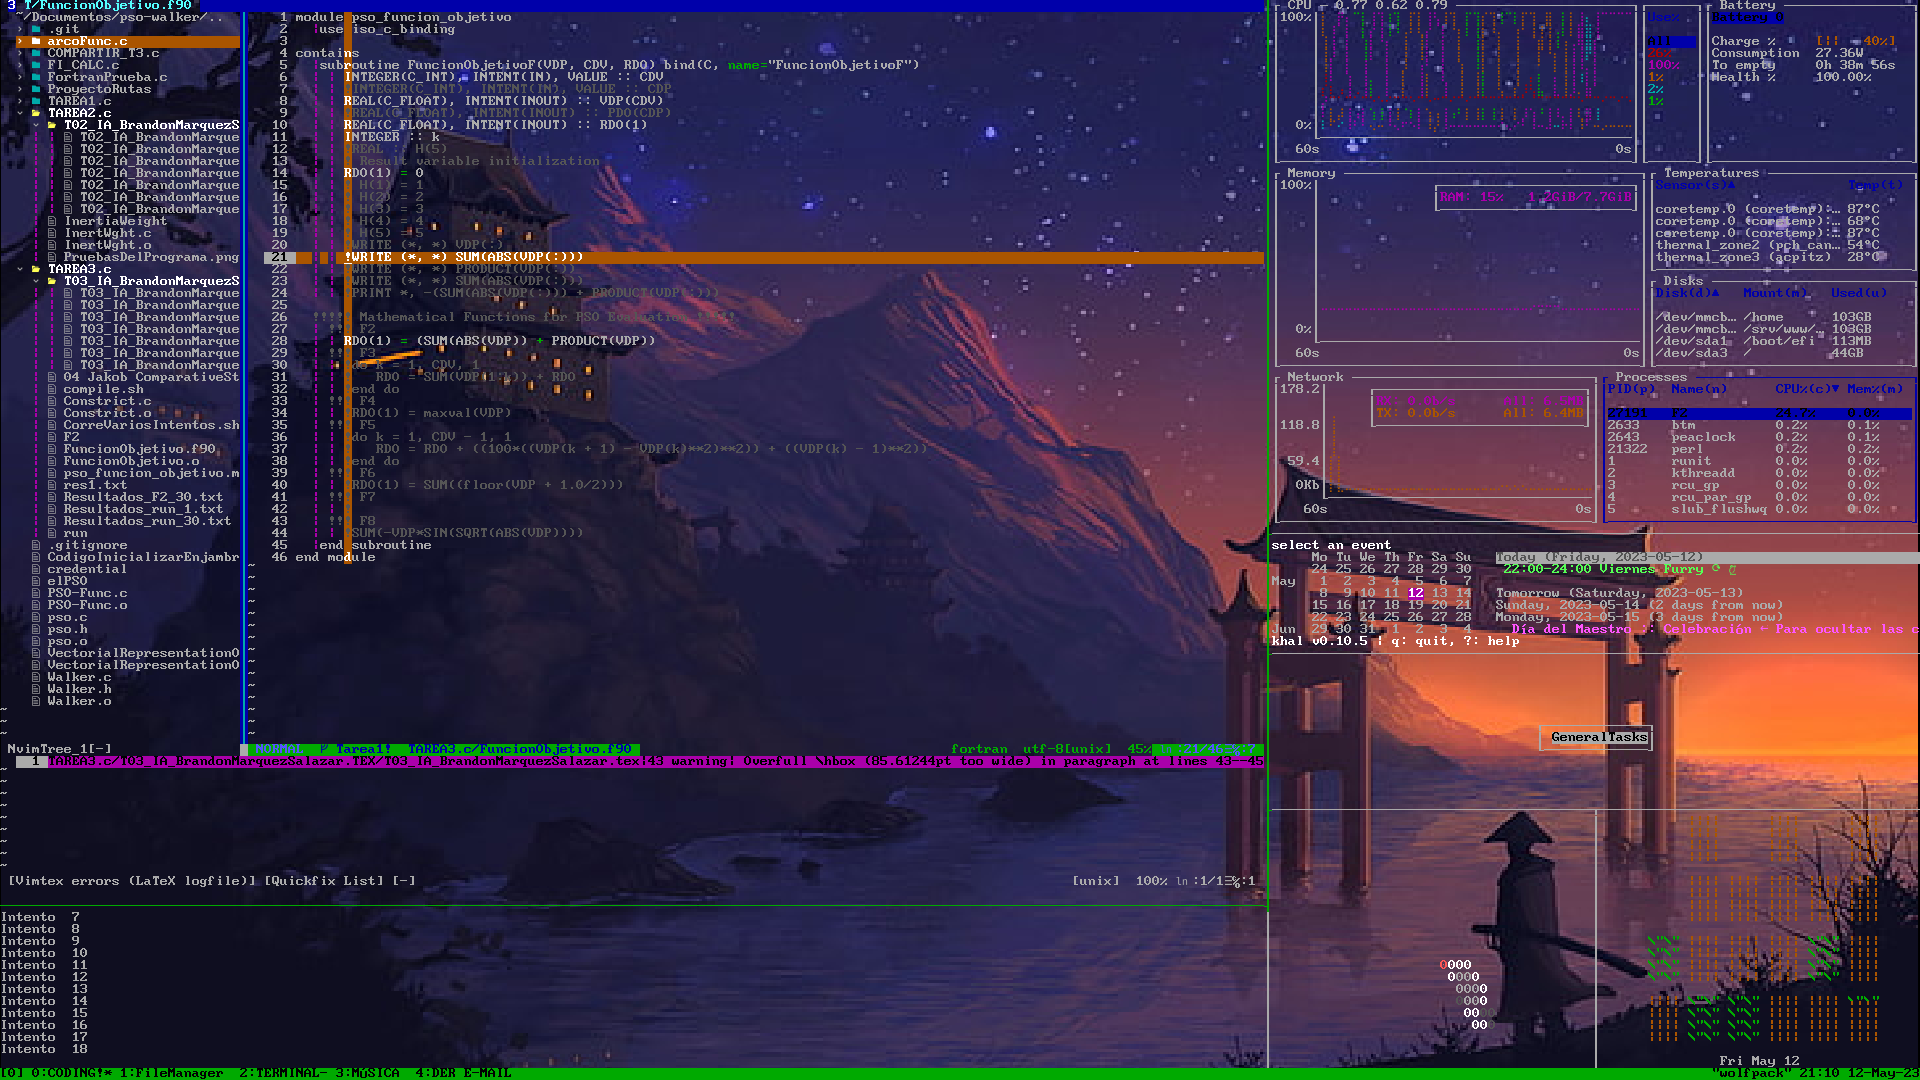
\includegraphics[scale=0.2]{PRUEBA.png}
  \subsection*{Datos de resultados}
  \parbox{2.4in}{\csvautotabular{../Resultados_F2_30.csv}}
  \parbox{3in}{
  Con un promedio de: 49.4i para Local Best\\ y un promedio de 0 para Global Best\\ Sin poder calcular la DevEst\newpage}
  \section*{Conclusión}
  El PSO con constricción impide la dispersión de un grupo de individuos, sin embargo, sus características matemáticas
  nos impide, también, una selección libre de los elementos C1 y C2, ya que la ecuación puede dar indeterminación, si
  acaso los valores no corresponden adecuadamente a la ecuación de constricción. Algo muy importante de plantear, es que
  se tuvo que sintonizar adecuadamente para evitar resultados extremos. El correrlo más de una vez, permitió observar
  el comportamiento y, estimando el promedio, verificar la precisión del método.
\end{document}
